% Sources :
%    * http://tex.stackexchange.com/questions/95077/help-for-one-simple-diagram-about-genetic-algorithmic
%    * http://tex.stackexchange.com/questions/95221/tikz-circled-arrow/95223#95223

\documentclass{article}
    \usepackage[utf8]{inputenc}
    \usepackage{tikz}
    \usetikzlibrary{arrows,shadows}

\def\circledarrow#1#2#3{ % #1 Style, #2 Center, #3 Radius
\draw[#1,->] (#2) +(80:#3) arc(80:-260:#3);
}

    \tikzset{
      frame/.style = {
        rectangle,
        draw,
        text width = 6em,
        text centered,
        minimum height=4em,drop shadow,fill=lime!40,
        rounded corners,
      },
      line/.style={
        draw, -latex',rounded corners=3mm,
      }
    }


\begin{document}

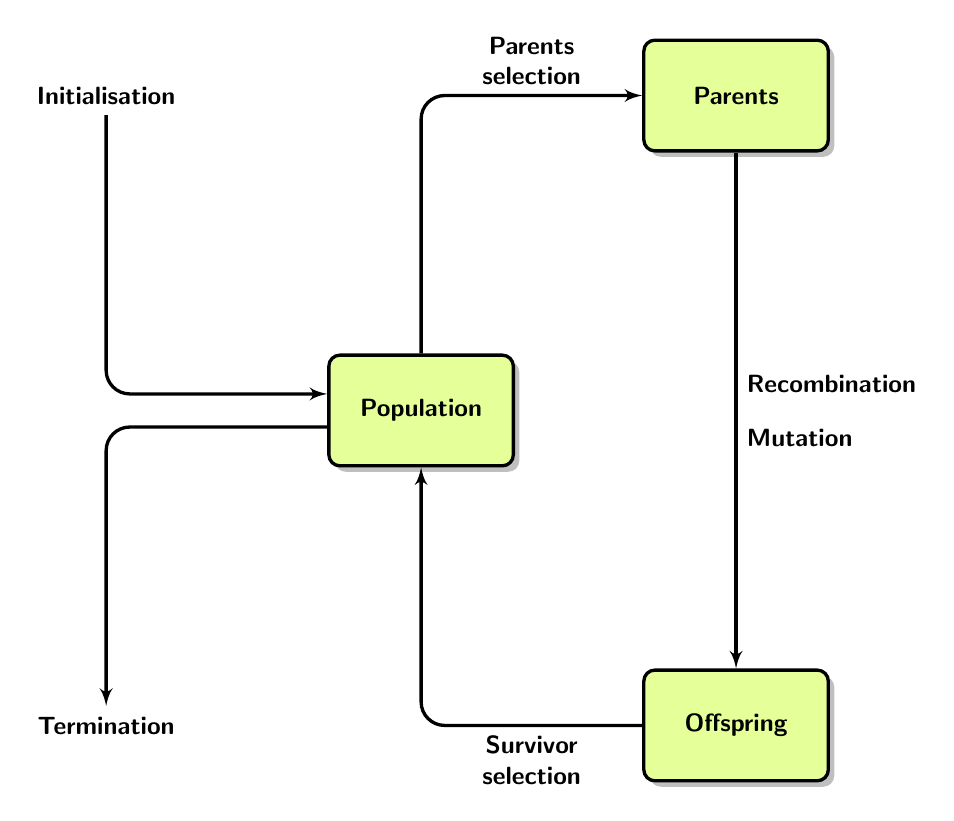
\begin{tikzpicture}[font=\small\sffamily\bfseries,very thick,node distance = 4cm]
    \node [frame] (pop) {Population};
    \node [above of=pop, left of=pop] (init) {Initialisation};
    \node [below of=pop, left of=pop] (term) {Termination};
    \node [frame, above of=pop, right of=pop] (parents)  {Parents};
    \node [frame, below of=pop, right of=pop] (off)  {Offspring};

    \path [line] (parents)
     -- node[right,align=left,pos=.5] {Recombination\\[3mm]Mutation}
     (off);
    \path [line] (init) |- (pop.170);
    \path [line] (pop.190) -| (term);
    \path [line] (off) -| node[below,pos=.25, align=center]
{Survivor\\ selection}(pop);
    \path [line] (pop) |- node[above,pos=.75, align=center]
{Parents\\ selection}(parents);
\end{tikzpicture}


\medskip
\hrule
\medskip


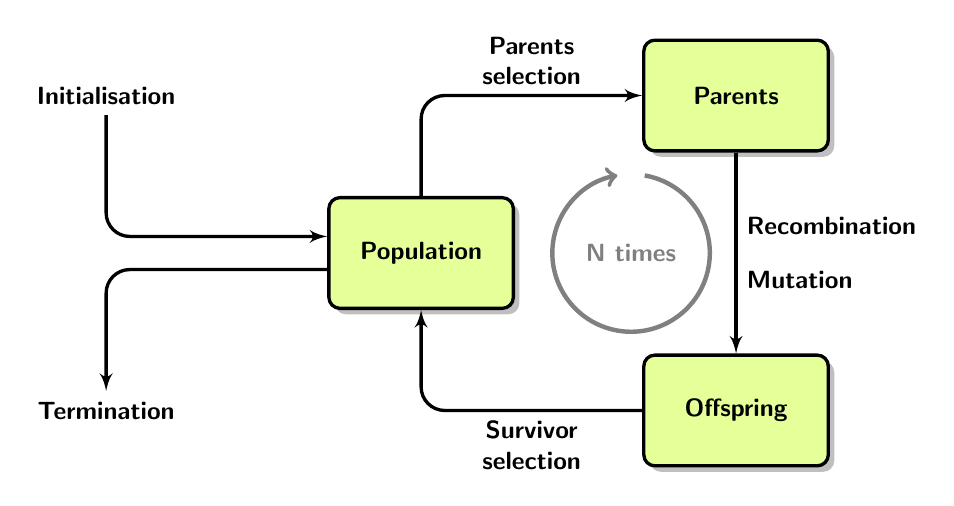
\begin{tikzpicture}[font=\small\sffamily\bfseries,very thick,node distance = 4cm]
    \node [frame] (pop) {Population};
    \node [above=2cm, left of=pop] (init) {Initialisation};
    \node [below=2cm, left of=pop] (term) {Termination};
    \node [frame, above=2cm, right of=pop] (parents)  {Parents};
    \node [frame, below=2cm, right of=pop] (off)  {Offspring};

    \path [line] (parents)
         -- node[right,align=left,pos=.5] {Recombination\\[3mm]Mutation}
        (off);
    \path [line] (init) |- (pop.170);
    \path [line] (pop.190) -| (term);
    \path [line] (off) -| node[below,pos=.25, align=center] {Survivor\\ selection}(pop);
    \path [line] (pop) |- node[above,pos=.75, align=center] {Parents\\ selection}(parents);

    \node at (barycentric cs:pop=1 ,parents=1 ,off=1) [color=gray] (insidetext) {N times};
    \circledarrow{ultra thick, gray}{insidetext}{1cm};
\end{tikzpicture}

\end{document}
